\chapter{Relational Data Model \& Relational Algebra} % Depth 0

\section{RDBMS}

\begin{itemize}
    \item Database Management System (DBMS) : a computer system for creating and maintaining databases
    \item Relational Database Management System (RDBMS) : databases which consists of \textit{tables} (relations)
\end{itemize}

\begin{figure}[H]
    \centering
    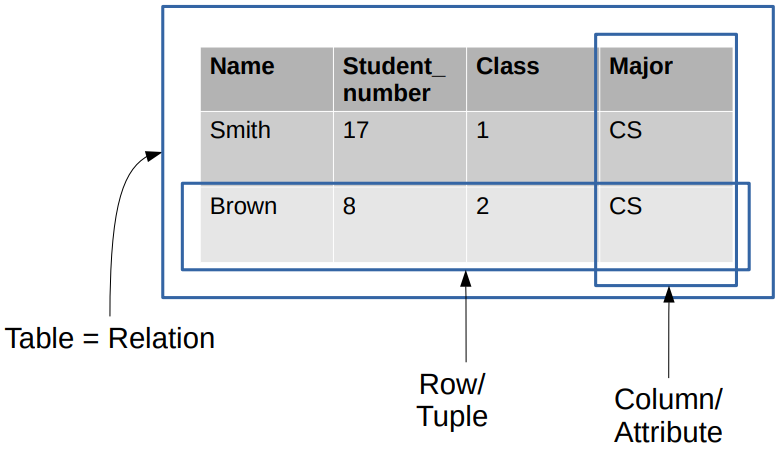
\includegraphics[width=0.6\textwidth,keepaspectratio]{RDBMS}
\end{figure}

\begin{Parallel}{0.47\textwidth}{0.47\textwidth}
\ParallelLText{
	\textgreen{\large{Pros}}
	\begin{itemize}
	    \item Ease of use due to abstraction (Logical/Physical independence)
	    \item Well known languages (SQL)
	    \item Reliability
	\end{itemize}
}

\ParallelRText{
	\textred{\large{Cons}}
	\begin{itemize}
	    \item Harder to obtain good performance, in particular in a distributed setting
	    \item Do not natively support very well some structures (Graph, Geographical data, Time-stamped data, ...)
	\end{itemize}
}
\ParallelPar
\end{Parallel}

\section{Relational Algebra}

Relational algebra is a set of mathematical rules and operators used to manipulate and query data in a relational database.

\subsection{Basic Operators}

\begin{itemize}
    \item \textblue{Selection} $\sigma_{\text{(<selection condition>)}}(R)$ : used to denote the \textit{SELECT} operator. The \textit{selection condition} is a boolean expression specified on the attributes of relation \textit{R}
        \begin{itemize}
            \item It is \textit{commutative} : $\sigma_{(\text{<cond1>)}}(\sigma_{(\text{<cond2>})}(R)) = \sigma_{(\text{<cond2>})}(\sigma_{(\text{<cond1>})}(R))$
            \item A cascade of selections can be combined : $\sigma_{(\text{<cond1>})}(\sigma_{(\text{<cond2>})}(...(\sigma_{(\text{<condn>})}(R))...)) =$ \\$\sigma_{\text{(<cond1> \textbf{AND} <cond2> \textbf{AND} ... \textbf{AND} <condn>})}(R)$
            \item In Rel : $\sigma_{(\text{Age}=20)}$(Student) = $\{t \in \text{Student} \ | \ t.\text{Age}=19 \}$
            \item In SQL : SELECT * FROM Student WHERE Age=20
        \end{itemize}
    \item \textblue{Projection} $\pi_{\text{<attributes>}}$ : selects a subset of columns from a table. The operation \textbf{removes any duplicate tuples}, so the result is a set of distinct tuples, and hence a valid relation (known as \textbf{duplicate elimination})
        \begin{itemize}
            \item In Rel : $\pi_{\text{Age}}$(Student) = $\{ t[\text{Age}] \ | \ t \in \text{Student} \}$
            \item In SQL : SELECT DISTINCT Age FROM Student
        \end{itemize}
    \item \textblue{Union} $(\cup)$ : combines two tables and eliminated duplicate rows (of the same type)
    \item \textblue{Intersection} $(\cap)$ : returns only the rows (of the same type) that appears in both tables
    \item \textblue{Difference} $(-)$ : returns the rows of one table that do not appear in another tables (the types need to correspond). Contratry to Union and Intersection, it is \textbf{not commutative}.
    \item \textblue{Cartesian product} $(\times)$ : combines every row of one table with every row of another table, creating a new table with all possible combinations of rows. For example, you could use cartesian products to create a table that combines all possible pairs of products and customers.
    \item \textblue{Division} $(\div)$ : The division operation is used to retrieve tuples from one relation that are related to all tuples in another relation. Here is an example:
        \begin{itemize}
            \item R contains information about students (A) and the subjects they are enrolled in (B)
            \item S contains a list of subjects (B)
            \item R ÷ S will retrieve the students (tuples from R) who are enrolled in all subjects (tuples from S)
            \item R has the following tuples: ('John', 'Math') ('John', 'English') ('Mary', 'Math') ('Mary', 'Science')
            \item S has the following tuple: ('Math')
            \item R ÷ S will be: ('John') ('Mary')
        \end{itemize}
    \item \textblue{Assignment} $(\leftarrow)$ : used to split an expression in several intermediate steps.\\Example : $\pi_{\text{Name}}(\text{(Student)} - \pi_{\text{Name}}(\text{(Follows)}$ is equivalent to :
        \begin{itemize}
            \item $S' \leftarrow \pi_{\text{Name}}(\text{(Student)}$
            \item $F' \leftarrow \pi_{\text{Name}}(\text{(Student)}$
            \item $S' - F'$
        \end{itemize}
    \item \textblue{General rename} $(\rho)$ : used to rename the attributes in the intermediate relations.\\Example : $\rho_{(\text{Name} \rightarrow \text{Name1})}(\text{Follows})$
\end{itemize}

\subsection{Join Operators}

The following "$\sigma_{A=B}(R_1 \times R_2)$" can be done using join operators as "$R_1 \bowtie_{A=B} R_2$"

\begin{itemize}
    \item \textblue{Theta join} $(\bowtie_{\theta})$ : combines tuples from two relations $R$ and $S$ based on a condition $\theta$ that involves attributes from both relations. The resulting relation contains all possible combinations of tuples from $R$ and $S$ \textit{that satisfy the condition}.
    \begin{itemize}
        \item \textblue{Equijoin} : special case of theta join where the condition is an equality comparison between attributes from the two relations. The resulting relation contains all possible combinations of tuples from R and S \textit{where the specified attributes are equal}.
    \end{itemize}
    \item \textblue{Natural join} $(\bowtie$ or $*)$ : performed between two relations with at least one common attribute. The join operation is done based on the common attribute(s) with the same name and domain in both relations. The resulting relation contains all possible combinations of tuples from $R$ and $S$ where the values of the common attributes are equal. Example :\\
    \begin{minipage}[t]{0.31\textwidth}
        \begin{center}
        \textgreen{Customer}\\
	    \begin{tabular}{|l|l|}
	    \hline 
	    Cid & Name \\ 
	    \hline 
	    \hline 
	    1 & Benjamin Bayer \\ 
	    \hline 
	    2 & Chung-cha Kim \\ 
	    \hline 
	    \end{tabular}
        \end{center}
    \end{minipage}
    \begin{minipage}[t]{0.31\textwidth}
        \begin{center}
        \textgreen{Buys}\\
	    \begin{tabular}{|l|l|}
	    \hline 
	    Cid & Pid \\ 
	    \hline 
	    \hline 
	    1 & A \\ 
	    \hline 
	    1 & B \\ 
	    \hline 
	    2 & B \\ 
	    \hline 
	    \end{tabular}
        \end{center}
    \end{minipage}
    \begin{minipage}[t]{0.31\textwidth}
        \begin{center}
        \textgreen{Product}\\
	    \begin{tabular}{|l|l|}
	    \hline 
	    Pid & Name \\ 
	    \hline 
	    \hline 
	    A & Cheese \\ 
	    \hline 
	    B & Milk \\ 
	    \hline 
	    \end{tabular}
        \end{center}
    \end{minipage}
    \begin{center}
    \textgreen{$\rho_{\text{Name} \rightarrow \text{CName}}(\text{Customer}) \bowtie \text{Buys} \bowtie \rho_{\text{Name} \rightarrow \text{PName}}(\text{Product})$}
    \begin{tabular}{|l|l|l|l|}
    \hline 
    Cid & CName & Pid & PName \\ 
    \hline
    \hline
    1 & Benjamin Bayer & A & Cheese \\ 
    \hline 
    1 & Benjamin Bayer & B & Milk \\ 
    \hline 
    2 & Chung-cha Kim & B & Milk \\ 
    \hline 
    \end{tabular} 
    \end{center}
    \newpage
    \item \textblue{Outer join} : includes all tuples from one or both participating relations, even if they do not satisfy the join condition. They are three types of outer joins :
    \begin{enumerate}
        \item \textblue{Left outer join} $(\leftouterjoin)$ : join that inserts \textit{NULL} for tuples missing in the second relation.
        \item \textblue{Right outer join} $(\rightouterjoin)$ : join that inserts \textit{NULL} for tuples missing in the first relation.
        \item \textblue{Full outer join} $(\fullouterjoin)$ : join that inserts \textit{NULL} for tuples missing in the other relation.
    \end{enumerate}
    \begin{minipage}[t]{0.48\textwidth}
        \begin{center}
        \textgreen{Customer}\\
	    \begin{tabular}{|l|l|}
	    \hline 
	    Cid & Name \\ 
        \hline
        \hline
	    1 & Benjamin Bayer \\ 
	    \hline 
	    2 & Chung-cha Kim \\ 
	    \hline 
	    3 & Barbara Benson \\ 
	    \hline 
	    \end{tabular}
        \end{center}
    \end{minipage}
    \begin{minipage}[t]{0.45\textwidth}
        \begin{center}
        \textgreen{Buys}\\
	    \begin{tabular}{|l|l|}
	    \hline 
	    Cid & Pid \\ 
        \hline
        \hline
	    1 & A \\ 
	    \hline 
	    1 & B \\ 
	    \hline 
	    2 & B \\ 
	    \hline 
	    4 & A \\ 
	    \hline 
	    \end{tabular}
        \end{center}
    \end{minipage}
    
    
    \smallskip
    \begin{minipage}[t]{0.3\textwidth}
        \begin{center}
        \textgreen{Customer $\leftouterjoin$ Buys}\\
        \begin{tabular}{|l|l|l|}
        \hline
        Cid & Name & Pid \\
        \hline
        \hline
        1 & B. Bayer & A \\
        \hline
        1 & B. Bayer & B \\
        \hline
        2 & C. Kim & B \\
        \hline
        3 & B. Benson & NULL \\
        \hline
        \end{tabular}
        \end{center}
    \end{minipage}
    \begin{minipage}[t]{0.3\textwidth}
        \begin{center}
        \textgreen{Customer $\fullouterjoin$ Buys}\\
        \begin{tabular}{|l|l|l|}
        \hline
        Cid & Name & Pid \\
        \hline
        \hline
        1 & B. Bayer & A \\
        \hline
        1 & B. Bayer & B \\
        \hline
        2 & C. Kim & B \\
        \hline
        3 & B. Benson & NULL \\
        \hline
        4 & NULL & A \\
        \hline
        \end{tabular}
        \end{center}
    \end{minipage}
    \begin{minipage}[t]{0.3\textwidth}
        \begin{center}
        \textgreen{Customer $\rightouterjoin$ Buys}\\
        \begin{tabular}{|l|l|l|}
        \hline
        Cid & Name & Pid \\
        \hline
        \hline
        1 & B. Bayer & A \\
        \hline
        1 & B. Bayer & B \\
        \hline
        2 & C. Kim & B \\
        \hline
        4 & NULL & A \\
        \hline
        \end{tabular}
        \end{center}
    \end{minipage}
\end{itemize}

\chapter{The Relational Model \& Integrity Constraints}

\section{Domain Constraints}

Every attribute has a domain, only values within the domain are allowed (i.e. \textit{VARCHAR, INT, CHAR, DATE}) and it is possible to explicitly allow/disallow \textit{NULL} for each attribute. It's also possible to restrict the range of allowed values, and define new types (based on existing types or enumerations).

Example :

\begin{minted}{sql}
CREATE DOMAIN SSN_TYPE AS CHAR(9):
CREATE DOMAIN D_NUM AS INT
    CHECK (Dnumber > 0 AND Dnumber < 21);
CREATE TYPE GENDER_TYPE AS ENUM ('M', 'F', 'N');

CREATE TABLE DEPARTMENT (
    Dname VARCHAR(15) NOT NULL,
    Dnumber D_NUM NOT NULL,
    Mgr_ssn SSN_TYPE NOT NULL,
    Mgr_start_date DATE );
\end{minted}

\section{Key Constraints}

\begin{itemize}
    \item \textblue{Superkey} : a set of one or more attributes that can uniquely identify a tuple (row) in a table. In other words, a superkey is a combination of one or more attributes that can garantee the uniqueness of each tuple in a table.
    \item \textblue{Key} : a minimal superkey; a superkey that has no other superkey as its subset.
    \item If a relation has multiple keys, all these keys are also called \textblue{candidate keys}. In database design it is common to indicate one the candidate keys as the \textblue{primary key}. The other candidate keys are \textblue{unique keys}.
    \item \textblue{Foreign key} : a field or combination of gields in one table that refers to the primary key of another table. It establish a relationship between two tables by ensuring referential integrity (meaning that data in one table is consistent with data in another table).
\end{itemize}

\section{Transaction}

Set of database operations that is executed in a manner that is \textblue{ACID} :
\begin{itemize}
    \item \textblue{A}tomic : After executing the transaction, all operations in the transaction have been executed, or none.
    \item \textblue{C}onsistent : After the transaction, all constraints are satisfied. Constraints are checked after all operations in the transaction have been executed, and all operations in the transaction are rejected if the result violates constraints.
    \item \textblue{I}solated : If multiple transactions are initiated at the same time, the database system will ensure that they are executed sequentially, such that one transaction is executed entirely before the other one is executed.
    \item \textblue{D}urable : If the database has indicated to a user program that it has finished executing a transaction, its results should be durable : the database remains in the correct state even in case of a power failure.
\end{itemize}

\chapter{Conceptual Modeling using Diagrams}

\section{Designing a Relational Database}

\subsection{Conceptual vs Physical Design}

\begin{minipage}[t]{0.48\textwidth}
\paragraph*{Conceptual design}
Visualization of the information that we conceptually plan to store; the decision how to link the tables to each other in the relational database is not made yet.
\end{minipage}
\hfill
\begin{minipage}[t]{0.48\textwidth}
\paragraph*{Physical design}
Every attribute in the relational database is listed, lines correspond exactly to foreign key relationships.
\end{minipage}

\begin{minipage}{0.48\textwidth}
\begin{figure}[H]
    \centering
    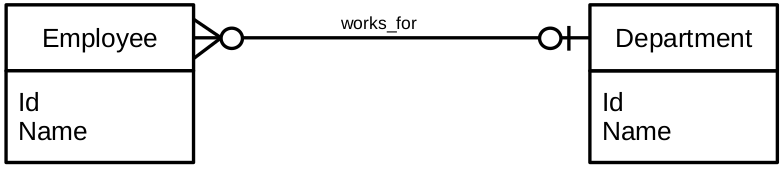
\includegraphics[width=\textwidth,keepaspectratio]{conceptual_d}
\end{figure}
\end{minipage}
\hfill
\begin{minipage}{0.48\textwidth}
\begin{figure}[H]
    \centering
    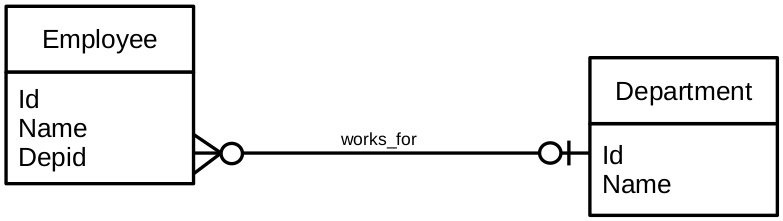
\includegraphics[width=\textwidth,keepaspectratio]{physical_d}
\end{figure}
\end{minipage}

\subsection{Different Types of Diagrams}

\begin{minipage}[t]{0.48\textwidth}
\paragraph*{Er-Chen}
\begin{itemize}
    \item Boxes for entities
    \item Diamonds for relationship
\end{itemize}
\end{minipage}
\hfill
\begin{minipage}[t]{0.48\textwidth}
\paragraph*{Crow's foot}
\begin{itemize}
    \item Boxes for entities
    \item Lines for relationship
\end{itemize}
\end{minipage}

\begin{minipage}{0.48\textwidth}
\begin{figure}[H]
    \centering
    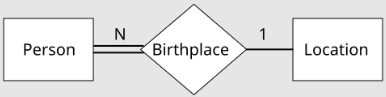
\includegraphics[width=\textwidth,keepaspectratio]{er-chen_example}
\end{figure}
\end{minipage}
\hfill
\begin{minipage}{0.48\textwidth}
\begin{figure}[H]
    \centering
    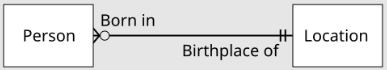
\includegraphics[width=\textwidth,keepaspectratio]{crow_foot_example}
\end{figure}
\end{minipage}

%
\begin{minipage}[t]{0.48\textwidth}
\paragraph*{Object Role}
\begin{itemize}
    \item Circles for objects
    \item Boxes for objects
\end{itemize}
\end{minipage}
\hfill
\begin{minipage}[t]{0.48\textwidth}
\paragraph*{UML}
\begin{itemize}
    \item Boxes for classes
    \item Lines for associations
\end{itemize}
\end{minipage}

\begin{minipage}{0.48\textwidth}
\begin{figure}[H]
    \centering
    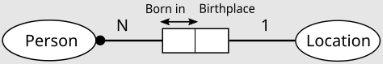
\includegraphics[width=\textwidth,keepaspectratio]{object_role_example}
\end{figure}
\end{minipage}
\hfill
\begin{minipage}{0.48\textwidth}
\begin{figure}[H]
    \centering
    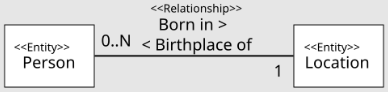
\includegraphics[width=\textwidth,keepaspectratio]{uml_example}
\end{figure}
\end{minipage}

\newpage
\subsection{Relationship Multiplicities}

\subsubsection{1:1 Multiplicity}

Refers to the number of occurrences of a relationship between two tables in database design. When a 1:1 multiplicity is not mandatory, it means that the relationship is optinal and not every record in one table need to be related to a record in the other table.

\begin{minipage}{0.45\textwidth}
\begin{figure}[H]
    \centering
    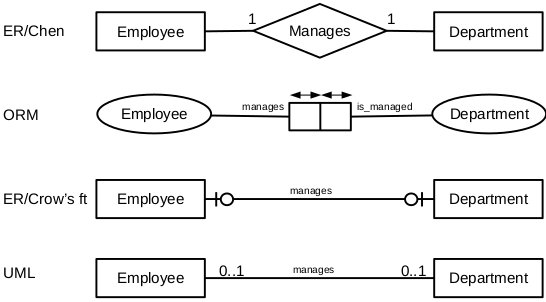
\includegraphics[width=0.7\textwidth,keepaspectratio]{1_1_mult_1}
\end{figure}
\end{minipage}
\hfill
\begin{minipage}{0.45\textwidth}
\begin{figure}[H]
    \centering
    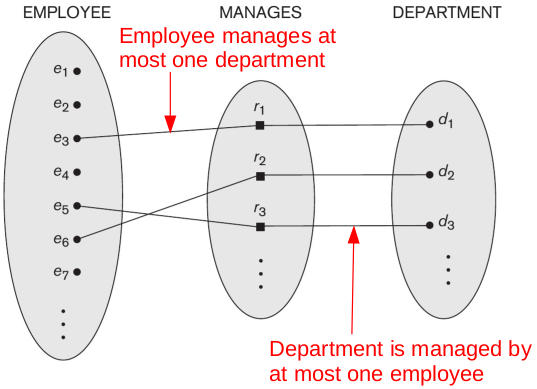
\includegraphics[width=0.65\textwidth,keepaspectratio]{1_1_mult_2}
\end{figure}
\end{minipage}


\subsubsection{M:N Multiplicity}

Refers to a many-to-many relationship between two tables. When a M:N multiplicity is not mandatory, it means that the relationship between the tables is optinal, and not every record in one table needs to be related to a record in the other table.

\begin{minipage}{0.45\textwidth}
\begin{figure}[H]
    \centering
    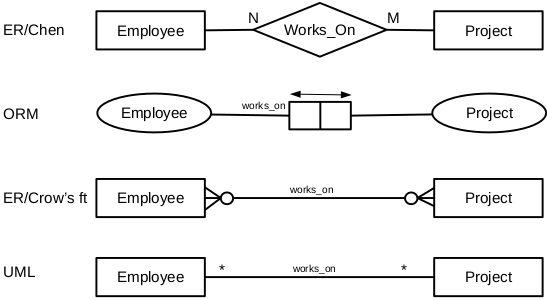
\includegraphics[width=0.7\textwidth,keepaspectratio]{M_N_mult_1}
\end{figure}
\end{minipage}
\hfill
\begin{minipage}{0.45\textwidth}
\begin{figure}[H]
    \centering
    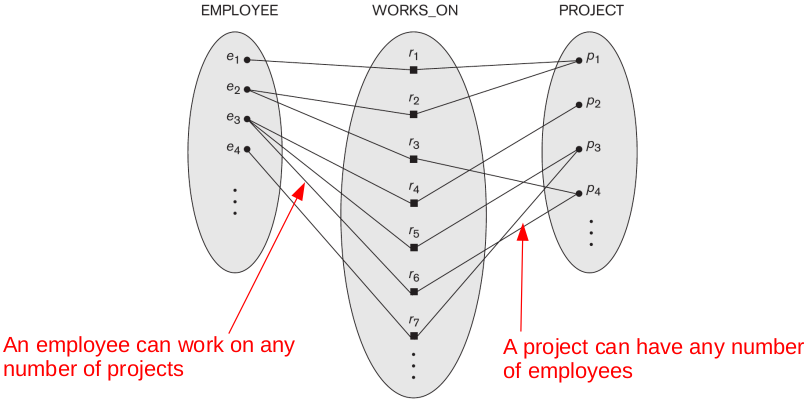
\includegraphics[width=0.8\textwidth,keepaspectratio]{M_N_mult_2}
\end{figure}
\end{minipage}

\subsubsection{1:N Multiplicity}

Refers to a one-to-many relationship between two tables

\begin{minipage}{0.45\textwidth}
\begin{figure}[H]
    \centering
    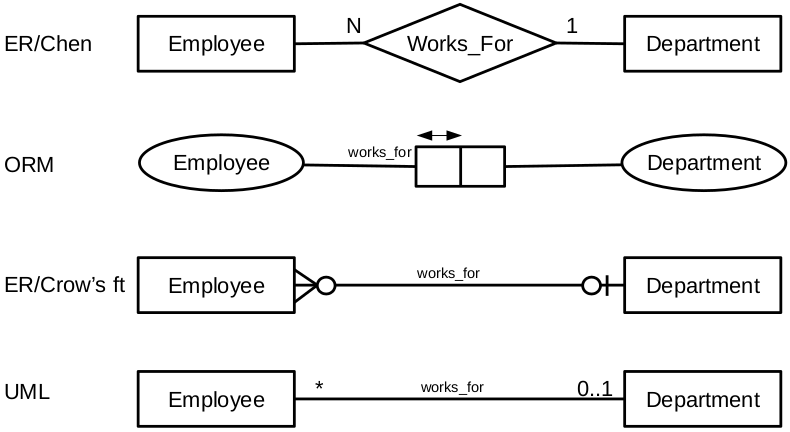
\includegraphics[width=0.7\textwidth,keepaspectratio]{1_N_mult_1}
\end{figure}
\end{minipage}
\hfill
\begin{minipage}{0.45\textwidth}
\begin{figure}[H]
    \centering
    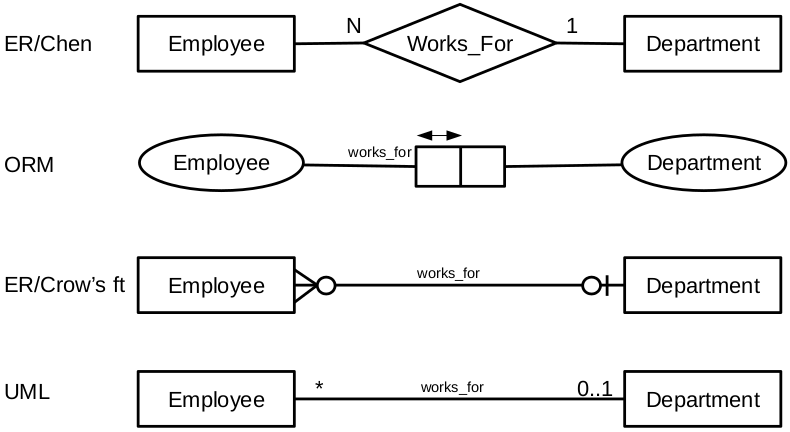
\includegraphics[width=0.8\textwidth,keepaspectratio]{1_N_mult_2}
\end{figure}
\end{minipage}

\subsubsection{1:N Multiplicity, Mandatory (left-handed)}

\begin{minipage}{0.45\textwidth}
\begin{figure}[H]
    \centering
    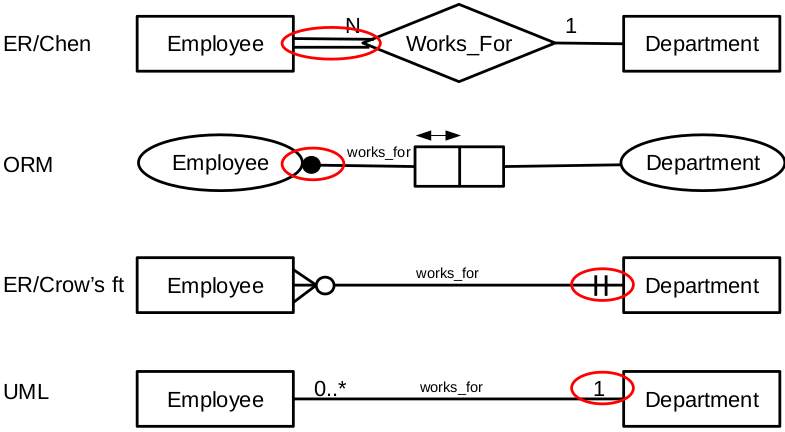
\includegraphics[width=0.7\textwidth,keepaspectratio]{1_N_mult_left_1}
\end{figure}
\end{minipage}
\hfill
\begin{minipage}{0.45\textwidth}
\begin{figure}[H]
    \centering
    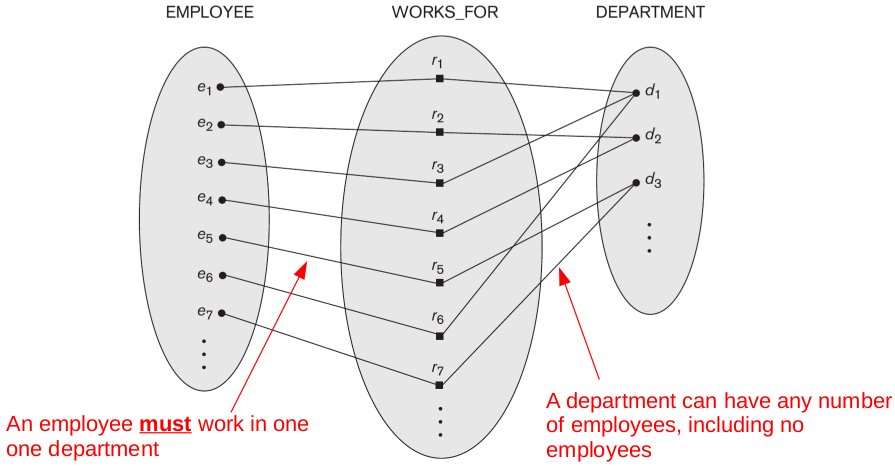
\includegraphics[width=0.8\textwidth,keepaspectratio]{1_N_mult_left_2}
\end{figure}
\end{minipage}

\subsubsection{1:N multiplicity, mandatory (both sides)}

\begin{minipage}{0.45\textwidth}
\begin{figure}[H]
    \centering
    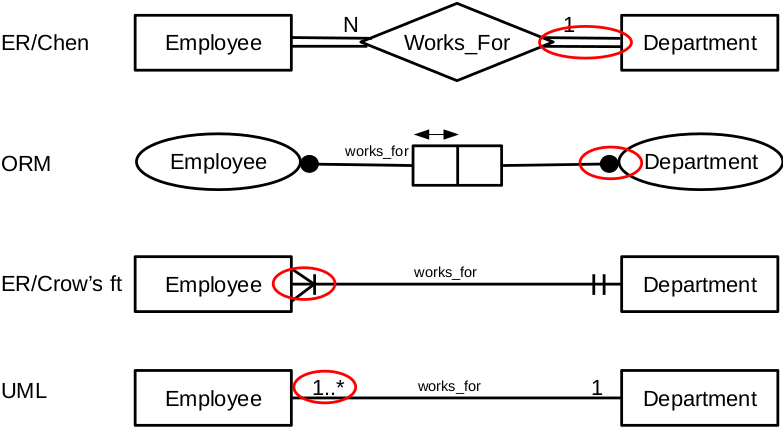
\includegraphics[width=0.7\textwidth,keepaspectratio]{1_N_mult_both_1}
\end{figure}
\end{minipage}
\hfill
\begin{minipage}{0.45\textwidth}
\begin{figure}[H]
    \centering
    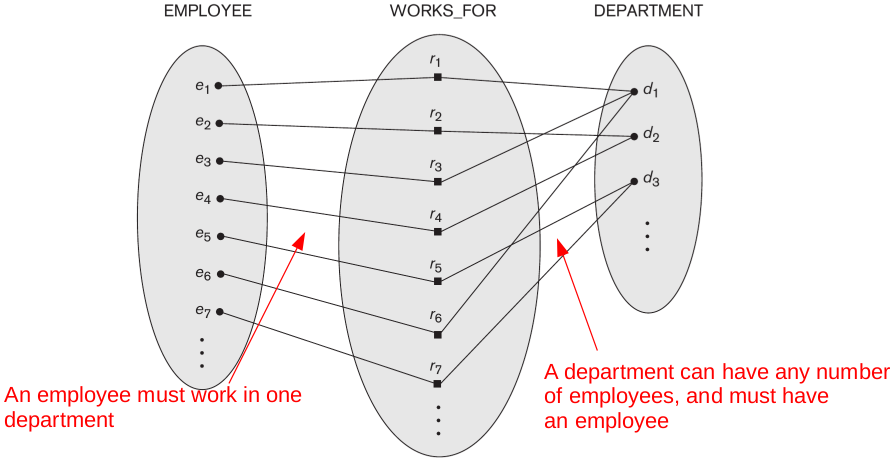
\includegraphics[width=0.8\textwidth,keepaspectratio]{1_N_mult_both_2}
\end{figure}
\end{minipage}

\subsubsection{Ternary Relationships}

Relationships between objects in three entities

\begin{minipage}{0.45\textwidth}
\begin{figure}[H]
    \centering
    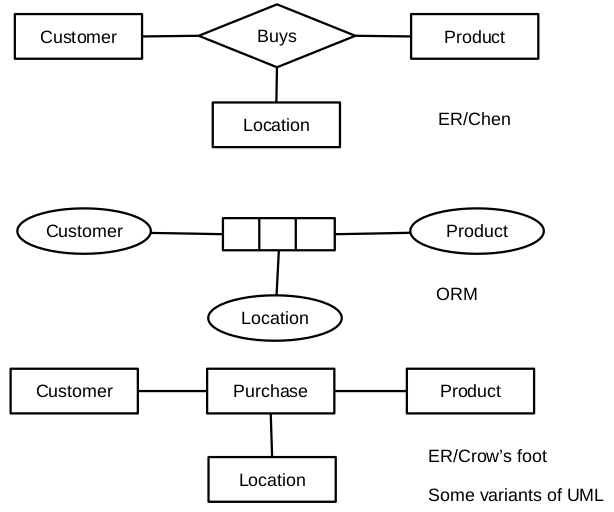
\includegraphics[width=0.8\textwidth,keepaspectratio]{ternary_1}
\end{figure}
\end{minipage}
\hfill
\begin{minipage}{0.45\textwidth}
\begin{figure}[H]
    \centering
    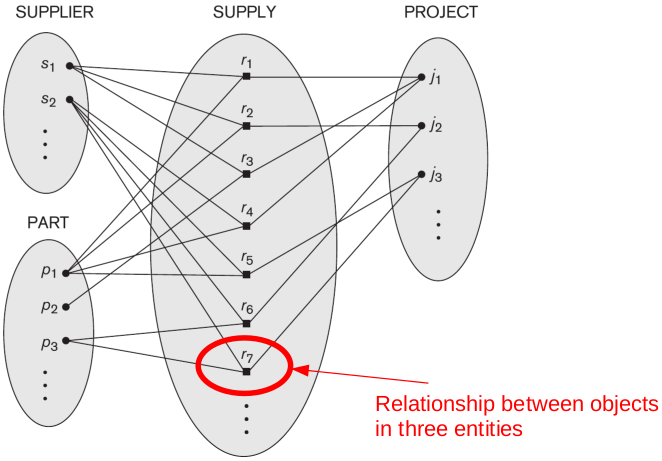
\includegraphics[width=0.8\textwidth,keepaspectratio]{ternary_2}
\end{figure}
\end{minipage}

\subsection{Attributes}

\subsubsection{Primary Keys}

\begin{minipage}[t]{0.32\textwidth}
\paragraph{Basics}
\begin{figure}[H]
    \centering
    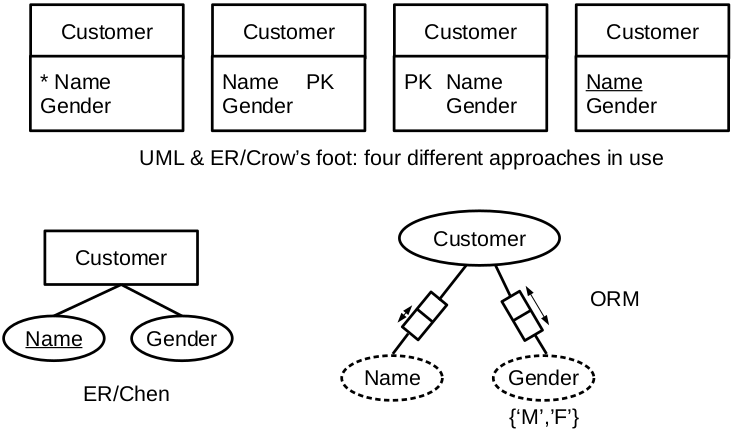
\includegraphics[width=\textwidth,keepaspectratio]{pk_b}
\end{figure}
\end{minipage}
\hfill
\begin{minipage}[t]{0.32\textwidth}
\paragraph{Composite keys}
\begin{figure}[H]
    \centering
    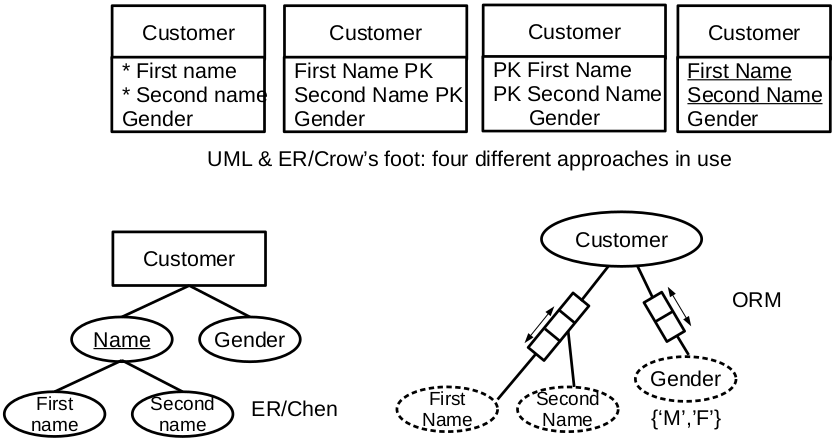
\includegraphics[width=\textwidth,keepaspectratio]{pk_ck}
\end{figure}
\end{minipage}
\hfill
\begin{minipage}[t]{0.32\textwidth}
\paragraph{Multiple keys}
\begin{figure}[H]
    \centering
    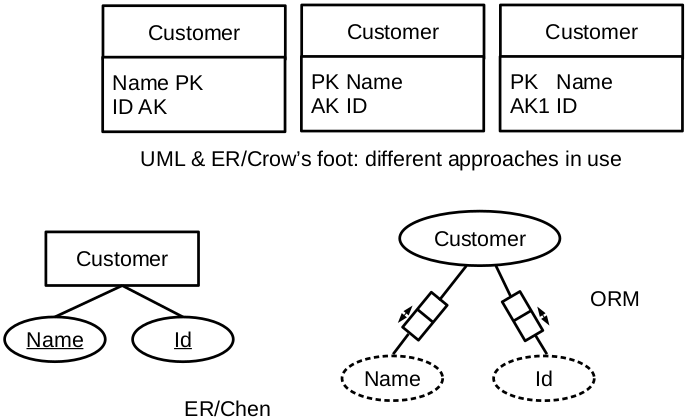
\includegraphics[width=\textwidth,keepaspectratio]{pk_mk}
\end{figure}
\end{minipage}

\subsubsection{Weak Entities}

Entities whose existence depends on the existence of another entify. In Er/Crow's foot notation, solid lines to indicate a relationship between an entity and a weak entity. Dashed lines for other relationships

\begin{minipage}{0.48\textwidth}
\begin{figure}[H]
    \centering
    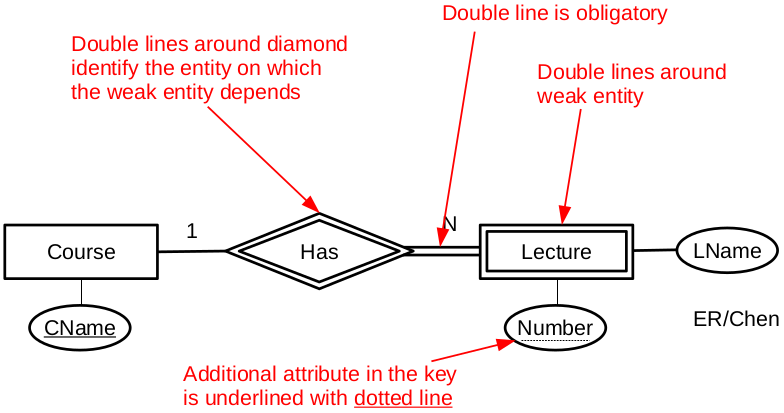
\includegraphics[width=\textwidth,keepaspectratio]{weak_entities_1}
\end{figure}
\end{minipage}
\hfill
\begin{minipage}{0.48\textwidth}
\begin{figure}[H]
    \centering
    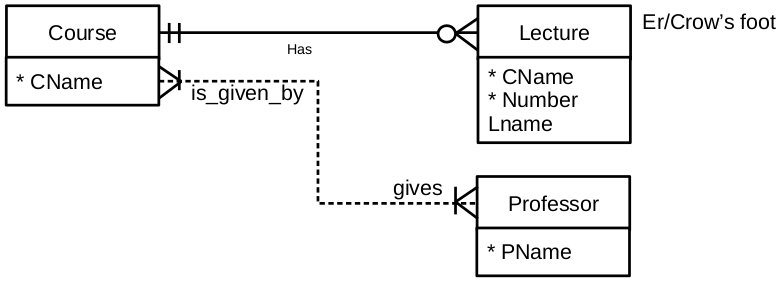
\includegraphics[width=\textwidth,keepaspectratio]{weak_entities_2}
\end{figure}
\end{minipage}

\section{Convertion ER/Chen Diagrams into Relational Schemas}

\begin{figure}[H]
    \centering
    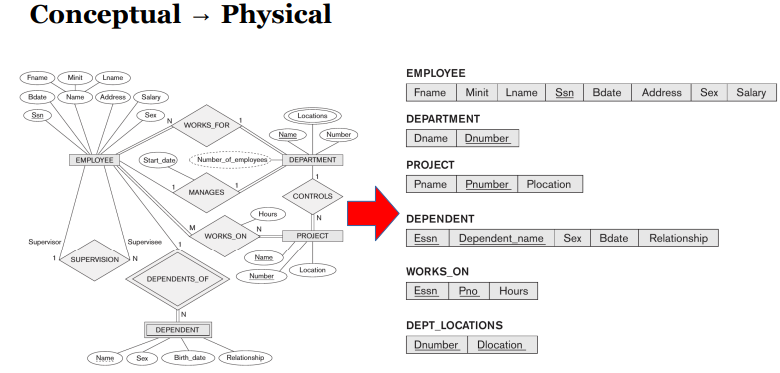
\includegraphics[height=6cm,keepaspectratio]{convertion_1}
\end{figure}

\subsection{Convert Entities}

\textblue{Convert the entities and all their single-valued attributes}

\begin{figure}[H]
    \centering
    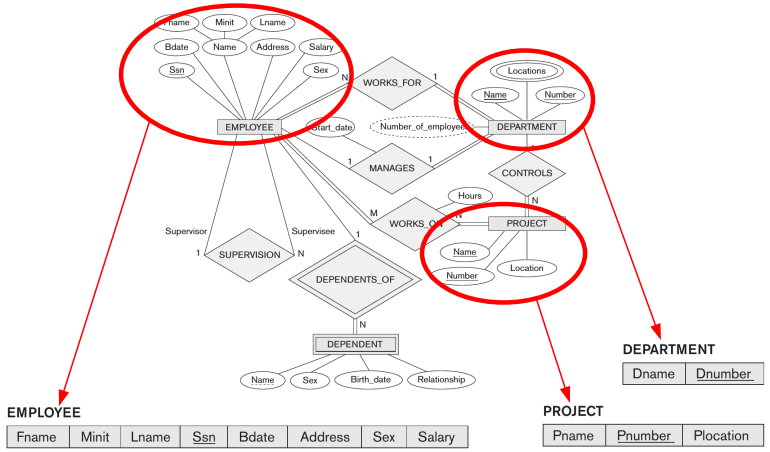
\includegraphics[height=6cm,keepaspectratio]{convertion_2}
\end{figure}

\subsection{Convert Weak Entities}

\textblue{Convert the weaker entities and all their single-valued attributes; add foreign key attributes for the owner entity type}

\begin{figure}[H]
    \centering
    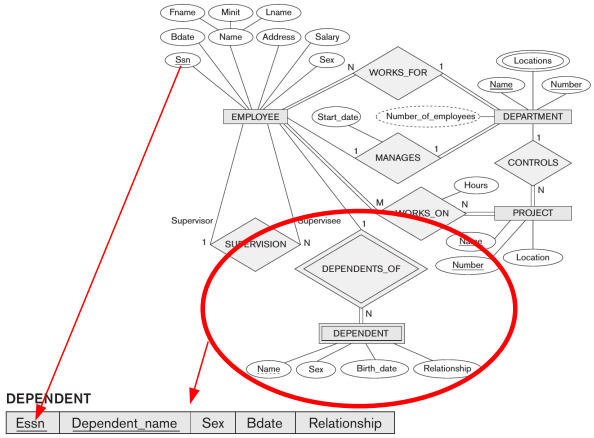
\includegraphics[height=7cm,keepaspectratio]{convertion_3}
\end{figure}

\subsection{Convert M:N Relations}

\textblue{Create an additional relation with foreign key attributes for the connected entities}

\begin{figure}[H]
    \centering
    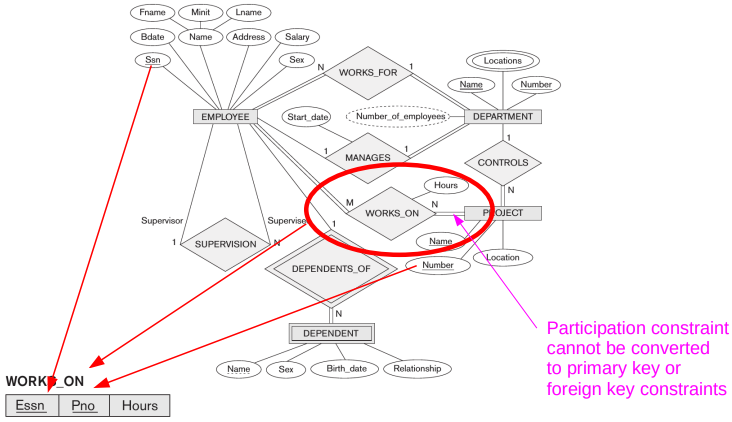
\includegraphics[height=6cm,keepaspectratio]{convertion_4}
\end{figure}

\subsection{Convert 1:1 Relations}

For each binary 1:1 relationship $R$, identify the relations $S$ and $T$ that correspond to the entity types participating in $R$. There are three possible approaches :

\begin{itemize}
    \item[] \textblue{Solution 1} : Use the same approach as for M:N relations.
        \begin{figure}[H]
            \centering
            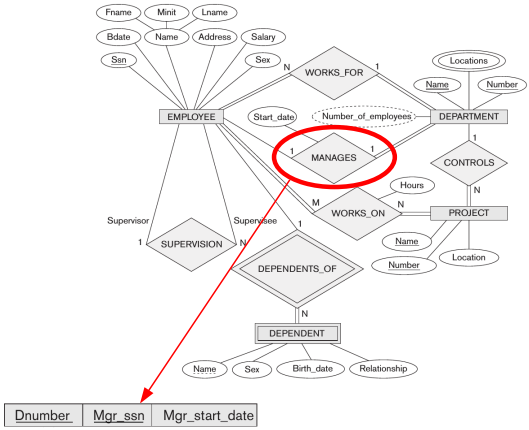
\includegraphics[height=6.5cm,keepaspectratio]{convertion_5}
        \end{figure}
    \item[] \textblue{Solution 2} : Add the key of one relation as a foreign key to the other.
        \begin{figure}[H]
            \centering
            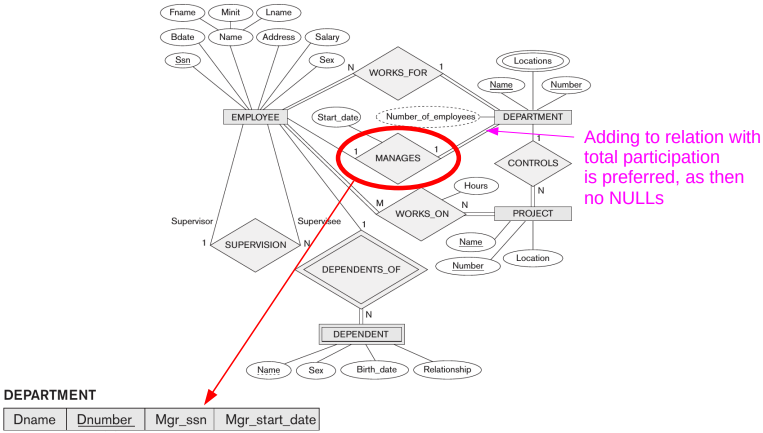
\includegraphics[height=6.5cm,keepaspectratio]{convertion_6}
        \end{figure}
    \item[] \textblue{Solution 3} : Merge the two connected relations.
        \begin{figure}[H]
            \centering
            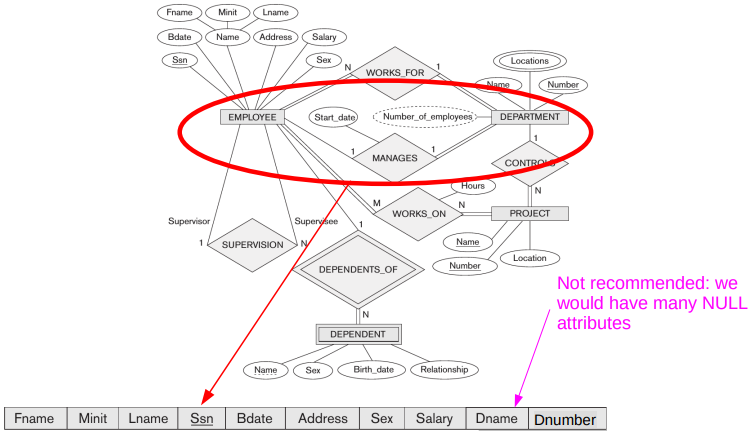
\includegraphics[height=6cm,keepaspectratio]{convertion_7}
        \end{figure}
\end{itemize}

\subsection{Convert 1:N Relations}

There are two possible approaches: 

\begin{itemize}
    \item[] \textblue{Solution 1} : Use the same approach as for M:N relations.
    \item[] \textblue{Solution 2} : Add the key of one relation as a foreign key to the other.
        \begin{figure}[H]
            \centering
            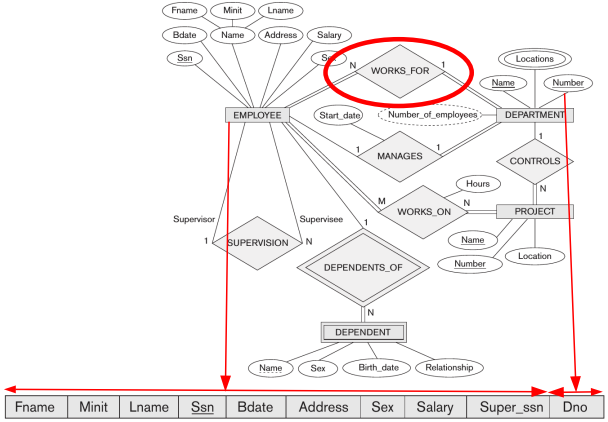
\includegraphics[height=7cm,keepaspectratio]{convertion_8}
        \end{figure}
\end{itemize}

\subsection{Convert Multi-Valued Attributes}

\textblue{Add a new relation for that attribute.}

\begin{figure}[H]
    \centering
    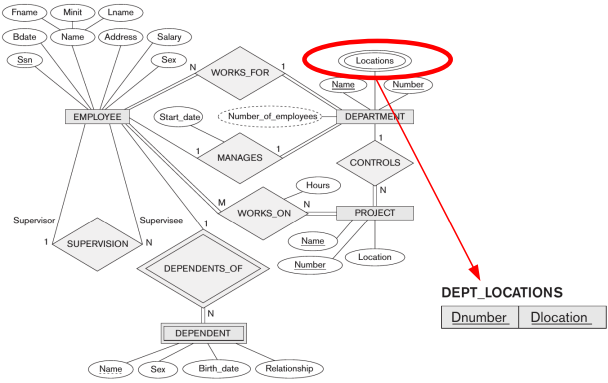
\includegraphics[height=6cm,keepaspectratio]{convertion_9}
\end{figure}

\subsection{Final Converted Schema}

\begin{figure}[H]
    \centering
    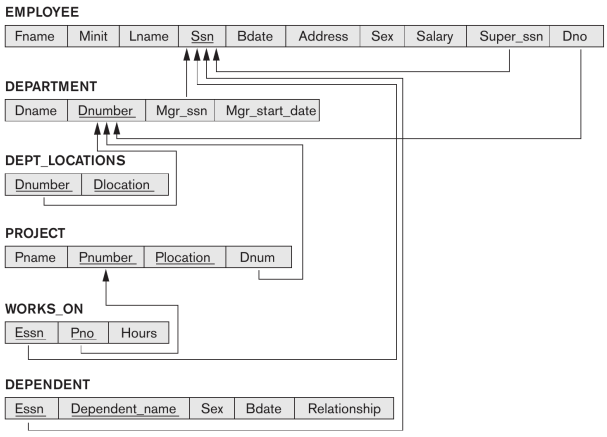
\includegraphics[height=6cm,keepaspectratio]{convertion_10}
\end{figure}

\chapter{Functional Dependencies \& Normal Forms}

\section{Normal Form Introduction}

A database design that satisfies formal properties are said to be in a normal form.

\subsection{First Normal Form}

\begin{itemize}
    \item Nested relations are not allowed; all values have to be atomic
    \item Repeating groups are not allowed (repetition of conceptually the same attribute)
\end{itemize}

\begin{figure}[H]
    \centering
    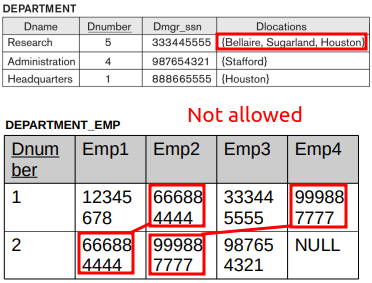
\includegraphics[height=5cm,keepaspectratio]{first_normal_form}
\end{figure}

\subsection{Second Normal Form}

\begin{minipage}[t]{0.48\textwidth}
\textred{Not allowed} in second normal form, as the table repeats information. If we change the name of a crouse, it would affect many rows.
\begin{figure}[H]
    \centering
    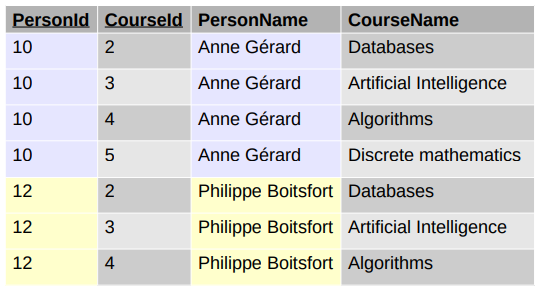
\includegraphics[width=0.8\textwidth,keepaspectratio]{second_normal_form_bad}
\end{figure}
\end{minipage}
\hfill
\begin{minipage}[t]{0.48\textwidth}
\textgreen{Good design} in second normal form. Information are not repeates, and changing a the name of a course would affect only one row.
\begin{figure}[H]
    \centering
    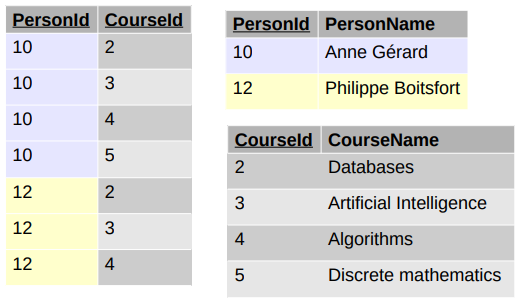
\includegraphics[width=0.8\textwidth,keepaspectratio]{second_normal_form_good}
\end{figure}
\end{minipage}

\section{Functional Dependencies}

Functional dependencies are relationships between attributes in a relational database table, where the value of one (\textit{dependent}) attribute is determined by the value of another (\textit{determinant}) attribute.

\subsection{Definition}

A \textblue{functional dependency} $X \rightarrow Y$ betqween sets of attributes $X$ and $Y$ in relation $R$, specifies a constraint that for any two tuples $t_1$ and $t_2$ in $R$ :

\begin{equation*}
\text{if } \forall A \in X : t_1.A = t_2.A \text{ then it holds that } \forall A \in Y : t_1.A = t_2.A
\end{equation*}

\newpage
\subsection{Classes of Functional Dependencies}

\begin{itemize}
    \item A functional dependency $X \rightarrow Y$ is called :
    \begin{itemize}
        \item \textblue{Full} if there is no $A \in X$ in such that $(X - \{A\}) \rightarrow Y$ is a functional dependency
        \item \textblue{Partial} otherwise
    \end{itemize}
    \item A functional dependency $X \rightarrow Y$ is called \textblue{trivial} if $Y \subseteq X$ 
\end{itemize}

For example, if we have a table of customer orders with attributes (\textit{order\_number, customer\_name, customer\_address}) and a functional dependency of \textit{customer\_name} $\rightarrow$ \textit{customer\_name}, this is a \textit{trivial} dependency since the information contained in the dependent attribute (\textit{customer\_name}) is already present in the determinant attribute (\textit{customer\_name}).

On the other hand, if we have a functional dependency of \textit{order\_number} $\rightarrow$ \textit{customer\_name}, this is a \textit{non-trivial} dependency since it provides new information about the relationship between orders and customers.

\subsection{Armstrong's Axioms}

\begin{itemize}
    \item The following axioms allow to derive FDs from given FDs, and are \textblue{sound} and \textblue{complete}
    \begin{enumerate}
        \item \textblue{Reflexive rule} : if $X \supseteq Y$, then $X \rightarrow Y$
        \item \textblue{Augmentation rule} : $X \rightarrow Y \models XZ \rightarrow YZ$
        \item \textblue{Transitive rule} : $X \rightarrow Y, Y \rightarrow Z \models X \rightarrow Z$
    \end{enumerate}
    \item Where,
    \begin{itemize}
        \item \textblue{Sound} = all FDs derived by using the rules are implied by the original set of FDs.
        \item \textblue{Complete} = all FDs that are implied by a set of FDs can be derived using these rules.
    \end{itemize}
\end{itemize}

Example :

Show that $A \rightarrow B \models AC \rightarrow B$

\begin{enumerate}
    \item $A \rightarrow B$ (Given)
    \item $AC \rightarrow BC$ (Augmentation rule on 1)
    \item $BC \rightarrow B$ (Reflexive rule)
    \item $AC \rightarrow B$ (Transitive rule on 2, 3)
\end{enumerate}

\section{Second Normal Form}

Every non-prime attribute (i.e., an attribute that is not part of any candidate key) must be fully functionally dependent on the primary key. This means that any attribute that is not part of the primary key must be dependent on the entire primary key, and not just part of it.

For example, consider a table of customer orders with attributes (\textit{order\_number, customer\_name,\\ item\_code, item\_description, quantity}). The primary key in this table is \textit{order\_number}. The \textit{item\_code} and \textit{item\_description} are non-prime attributes since they are not part of the primary key.

To satisfy \textit{2NF}, we must ensure that the \textit{item\_code} and \textit{item\_description} are fully functionally dependent on the \textit{order\_number}. This means that for any given \textit{order\_number}, there should be only one \textit{item\_code} and one \textit{item\_description}. If there are multiple \textit{item\_code} or \textit{item\_description} associated with a single \textit{order\_number}, this would violate \textit{2NF} and could lead to data anomalies such as redundancy and inconsistency.

To determine whether a table with given sets of functional dependencies is in \textit{2NF}, you can follow these step-by-step guidelines:

\begin{enumerate}
    \item Identify the candidate keys:
    \begin{itemize}
        \item Look for functional dependencies where the left-hand side is a superkey (a set of attributes that uniquely identifies a tuple).
        \item Candidate keys can be derived from such superkeys.
        \item If there are multiple candidate keys, choose one for analysis.
    \end{itemize}
    \item Examine the functional dependencies for partial dependencies:
    \begin{itemize}
        \item Check if any non-prime attribute (attribute not part of the candidate key) depends on only a part of the candidate key.
        \item If such partial dependencies exist, the table is \textblue{not in \textit{2NF}}.
        \item Should have a candidate key that includes the determinant attribute(s).
    \end{itemize}
    \item Examine the functional dependencies for transitive dependencies:
    \begin{itemize}
        \item Check if any non-prime attribute depends on another non-prime attribute (i.e., a non-key attribute).
        \item If transitive dependencies exist, the table is \textblue{not in \textit{2NF}}.
        \item Attribute is fully functionally dependent on the entire candidate key(s).
    \end{itemize}
\end{enumerate}

By following these steps, you can assess whether a table with the given sets of functional dependencies is in \textit{2NF}. Remember to consider the primary keys derived from the functional dependencies when evaluating the normalization form.

\begin{minipage}[b]{0.48\textwidth}
\begin{figure}[H]
    \centering
    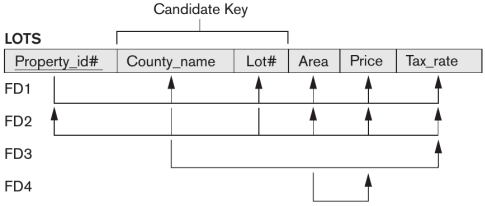
\includegraphics[width=\textwidth,keepaspectratio]{2nf_example_1}
    \caption{This relation is \textred{not} in \textit{2NF}}
\end{figure}
\end{minipage}
\hfill
\begin{minipage}[b]{0.48\textwidth}
\begin{figure}[H]
    \centering
    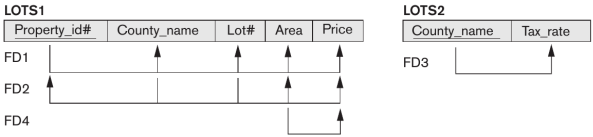
\includegraphics[width=\textwidth,keepaspectratio]{2nf_example_2}
    \caption{These relation are in \textit{2NF}}
\end{figure}
\end{minipage}

\section{Third Normal Form}

A relation is in third normal form iff for every nontrivial full functional dependency in $X \rightarrow A$ in $R$ :
\begin{itemize}
    \item either $X$ is a key
    \item or $A$ is a prime attribute
\end{itemize}

If a relation is in third normal form, it is also in second normal form.

Essentially, this means that in a 3NF relation, every nontrivial functional dependency involves either the key attributes or attributes that are directly dependent on the key attributes. This helps to eliminate redundancy and ensure data integrity.

\begin{figure}[H]
    \centering
    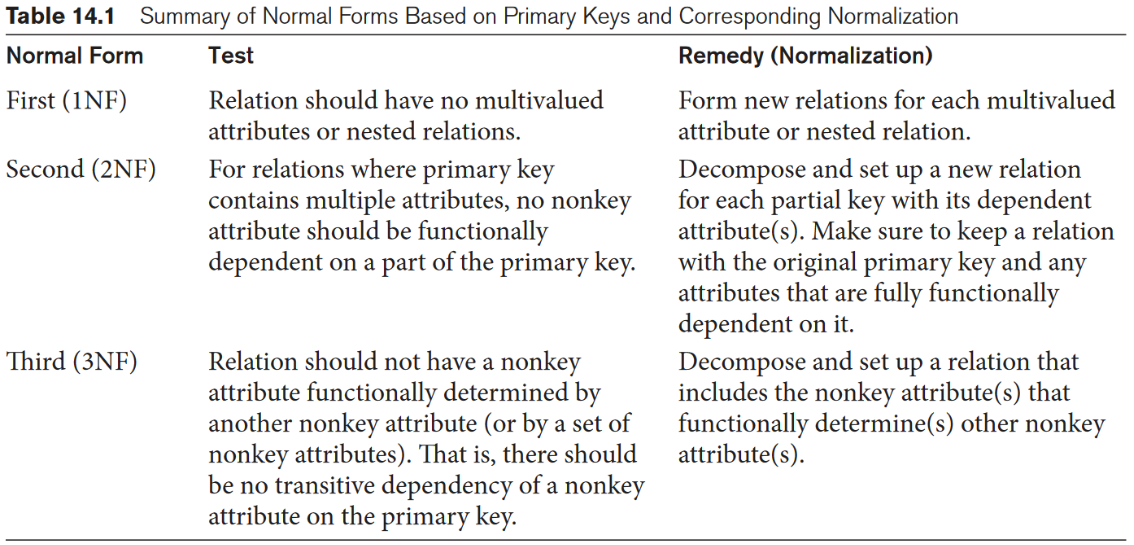
\includegraphics[width=\textwidth,keepaspectratio]{nf_summary}
\end{figure}

\section{Full Functional Dependencies}

Refer to dependencies where removing any attribute from the dependency would result in a loss of functionality. Non-trivial functional dependencies, on the other hand, imply that the dependent attribute cannot be determined by a trivial rule or a subset of attributes.

To identify full and non-trivial functional dependencies in a table, we need to examine the relationships between the attributes based on their values. Here's an example table to illustrate the concept:

\begin{center}
\begin{tabular}{|c|c|c|c|}
\hline
A & B & C & D \\ 
\hline 
\hline
a1 & b1 & c1 & d1 \\ 
\hline 
a1 & b2 & c2 & d1 \\ 
\hline 
a2 & b1 & c2 & d2 \\ 
\hline 
a2 & b1 & c2 & d2 \\ 
\hline 
\end{tabular} 
\end{center}

Let's analyze the functional dependencies:

\begin{enumerate}
    \item $A, B \rightarrow C, D$: This is a full and non-trivial functional dependency because given the values of $A$ and $B$, we can uniquely determine the values of $C$ and $D$. Removing either $A$ or $B$ would break the dependency.
    \item $B \rightarrow C$: This is also a full and non-trivial functional dependency because given the value of $B$, we can determine the value of $C$. Removing B would break the dependency.
\end{enumerate}

In summary, the table exhibits full and non-trivial functional dependencies between the attributes $A$, $B$, $C$, and $D$.

\chapter{Indexing}

\section{Disk Memory}

\begin{minipage}{0.48\textwidth}
	\begin{figure}[H]
		\centering
		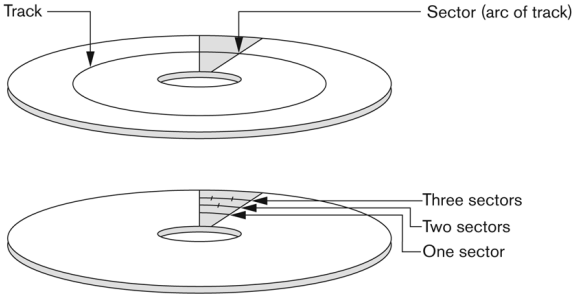
\includegraphics[width=\textwidth,keepaspectratio]{disks}
	\end{figure}
\end{minipage}
\hfill
\begin{minipage}{0.5\textwidth}
	\begin{itemize}
	    \item Hardware is only able to read/write an entire block
	    \item It is beneficial to store information that is often accessed together, within the same block
	    \item Record (tuples) are variable in length.
	    \begin{itemize}
	        \item Length of a field is indicated before the field
	        \item Special code at the end
	        \item Can span multiple blocks if they are too long to fit in 1 block
	    \end{itemize}
	\end{itemize}
\end{minipage}

\section{Records}

\subsection{Unordered Records}

\begin{minipage}[t]{0.48\textwidth}
\textgreen{Advantages}
\begin{itemize}
    \item Relatively easy to insert a record in the\\ database (if duplicates are allowed : put the new record at the end of the data file)
    \item Relatively simple to implement
\end{itemize}
\end{minipage}
\hfill
\begin{minipage}[t]{0.48\textwidth}
\textred{Disadvantages}
\begin{itemize}
    \item Searching for records is time consuming
    \item Listing the records in a desired order can be time consuming
\end{itemize}
\end{minipage}

\subsection{Ordered Records}

\begin{minipage}[t]{0.48\textwidth}
\textgreen{Advantages}
\begin{itemize}
    \item Relatively easy to find a particular record (binary search)
    \item Relatively simple to list records
\end{itemize}
\end{minipage}
\hfill
\begin{minipage}[t]{0.48\textwidth}
\textred{Disadvantages}
\begin{itemize}
    \item Inserting records is difficult
    \item Deleting records is difficult
\end{itemize}
\end{minipage}

\section{Indexes}

Indexes are data structures that make it more efficient to search for desired records.

\subsection{Single-level Indexes}

\subsubsection{Primary Indexes}

\begin{itemize}
    \item Defined on an ordered data file
    \item Datafile is ordered on a key attribute
    \item A primary index is a \textblue{nondense (sparse) index} : the index does not contain a pointer to every tuple present in the data file
\end{itemize}

\subsubsection{Clustering Indexes}

\begin{itemize}
    \item Defiend on an ordered data file
    \item Distinguishing feature : the data file can also be ordered a non-key field (multiple records can have the same value)
    \item A clustering index is also a nondense (sparse) index, when defined on non-key attributes
\end{itemize}

\subsubsection{Secondary Indexes}

\begin{itemize}
    \item Provides a secondary means of accessing a file for which some primary access already exists
    \item The index is an ordered file with two fields:
    \begin{itemize}
        \item The first field contains the indexed attribute
        \item The second field is either a block pointer or a record pointer
    \end{itemize}
    \item Unlike a primary index, a secondary index is usually dense, meaning that it contains an entry for every record in the file
    \item Listing records in order using a secondary index can be time-consuming
\end{itemize}

\subsection{Multi-level Index}

\begin{itemize}
    \item As a first-level index is ordered, one can also build an \textblue{index on the index} to obtain  amulti-level index
    \item Consist of a tree
\end{itemize}

\subsubsection{B+-Trees}

\begin{itemize}
    \item Trees in which each node occupies one block on disk
    \item Each internal node can contain multiple (key) values and pointers to other index blocks
    \item Leafs contain pointers to data blocks
    \item Aim to make insertion/deletion easier
    \item Not necessarily full, each node is only between half full and completely full
\end{itemize}

\begin{figure}[H]
    \centering
    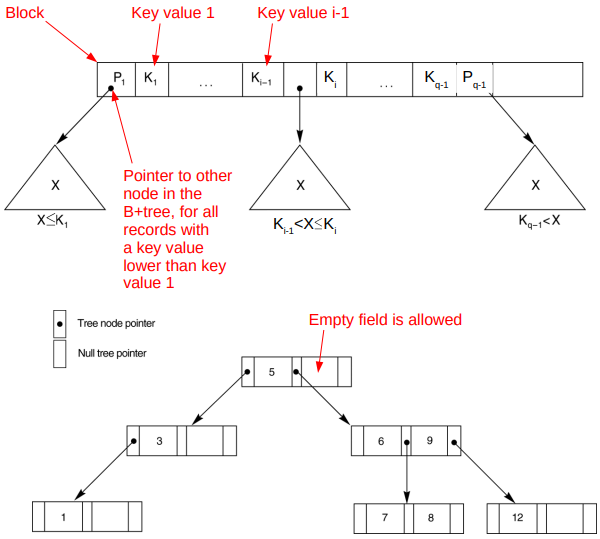
\includegraphics[height=8cm,keepaspectratio]{b+-_tree}
\end{figure}

\begin{minipage}[t]{0.48\textwidth}
\paragraph{Insertion}
\begin{itemize}
    \item Search the leaf index block in which the record pointer should be stored
    \item If the index block has space left, write an updated index block to disk
    \item If the index block has no space left, splut the block into two, and recursively update the parent block
\end{itemize}
\end{minipage}
\hfill
\begin{minipage}[t]{0.48\textwidth}
\paragraph{Deletion}
\begin{itemize}
    \item Search the leaf block from which the record should be removed
    \item If the block is less than half full after the removal of the record:
    \begin{itemize}
        \item Redistribute some values from a neighboring block, as long as this neighboring block is more than half-full
        \item Merge the block with a neighboring block if it is half-full as well
        \item Update changes upwards
    \end{itemize}
\end{itemize}
\end{minipage}

\subsubsection{B-Trees}

\begin{itemize}
    \item Variation of \textit{B+-Trees} in which internal nodes also stores pointers to data record.
    \item Leaf nodes and internal nodes have similar structure.
\end{itemize}

\begin{figure}[H]
    \centering
    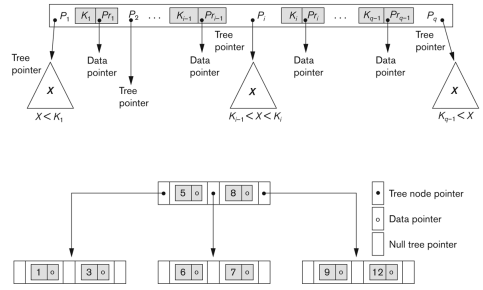
\includegraphics[height=6cm,keepaspectratio]{b-_tree}
\end{figure}

\subsubsection{B-Tress vs B+-Trees}

\begin{minipage}[t]{0.48\textwidth}
\paragraph{Advantages of B-Trees}
\begin{itemize}
    \item One could try to put frequently accessed values closer to the root of the tree, making search for those values faster
    \item Simpler implementation: all nodes the same
\end{itemize}
\end{minipage}
\hfill
\begin{minipage}[t]{0.48\textwidth}
\paragraph{Advantages of B+-Trees}
\begin{itemize}
    \item More key values fit into internal nodes
    \begin{itemize}
        \item B+-Trees are shallower (less levels)
        \item More efficient search for values in leafs (less blocks need to be fetched)
    \end{itemize}
    \item Listing in order is more efficient (follow pointers between leafs)
\end{itemize}
\end{minipage}

\subsection{Index In SQL}

\begin{itemize}
    \item Creating an index is simple :
    \begin{minted}{sql}
    CREATE INDEX salary_index ON EMPLOYEES (salary);
    \end{minted}
    \item Most databases will create either a B+- Tree or a B-Tree
    \item Indexes can also be used to maintain constraints. A unique index ensures that no two tuples have the same value :
    \begin{minted}{sql}
    CREATE UNIQUE INDEX salary_index ON EMPLOYEES (salary);
    \end{minted}
    \item It's important to note that for an index to be effectively used in a query, the conditions must match the index attributes from the leftmost position or as a prefix.
    \begin{minted}{sql}
    CREATE INDEX W ON TC(a,b,c);
    \end{minted}
    \begin{minipage}[t]{0.4\textwidth}
    \textgreen{Good pratice :}
    \begin{minted}{sql}
    SELECT *
    FROM TC C
    WHERE C.a = 1 AND C.b = 2;
    \end{minted}
    \end{minipage}
    \hfill
    \begin{minipage}[t]{0.4\textwidth}
    \textred{Bad pratice :}
    \begin{minted}{sql}
    SELECT *
    FROM TC C
    WHERE C.b = 1 AND C.c = 2;
    \end{minted}
    \end{minipage}
    \item In the case of an \textit{inequality condition}, the index allows for effective range scans or seek operations to locate the desired tuples based on the specified condition.
    \begin{minted}{sql}
    CREATE INDEX W ON TC(a,b,c);
    \end{minted}
    \begin{minipage}[t]{0.4\textwidth}
    \textgreen{Good pratice :}
    \begin{minted}{sql}
    SELECT *
    FROM TC C
    WHERE C.a > 1;
    \end{minted}
    \end{minipage}
    \hfill
    \begin{minipage}[t]{0.4\textwidth}
    \textred{Bad pratice :}
    \begin{minted}{sql}
    SELECT *
    FROM TC C
    WHERE C.b > 1;
    \end{minted}
    \end{minipage}
\end{itemize}

\subsubsection{Specific Behavior Of SQL Indexes}

\begin{itemize}
    \item It automatically adds a \textit{rowid} key to every tuple. If a value is not specified, SQLite will fill in a value for this attribute automatically
    \item If an integer primary key is defined, that integer attribute will be an alias for \textit{rowid} (and the other way around)
    \item It build a B+-tree for every relation, using the \textit{rowid} as key
\end{itemize}

\chapter{Relational Databases : Database Programming Techniques}

\section{Embedded SQL}

\begin{itemize}
    \item Extend common programming languages with syntax allowing to \textit{embed} SQL
    \item Uses a \textit{precompiler} : a tool that tranform source code with embedded SQL into source code without embedded SQL, replacing the embedded code with function calls
    \item Example using SQLJ for embedding SQL in Java :
    \begin{minted}[breaklines]{Java}
    ssn = readEntry("Enter a Social Security Number: ") ;
    try {
        #sql { SELECT Fname, Minit, Lname, Address, Salary
            INTO :fname, :minit, :lname, :address, :salary
            FROM EMPLOYEE WHERE Ssn = :ssn} ;
    } catch (SQLException se) {
        System.out.println("SSN does not exist: " + ssn) ;
        return;
    }
    System.out.println(fname + " " + minit + " " + lname + " " + address + " " + salary);
    \end{minted}
\end{itemize}

\section{Libraries}

\begin{itemize}
    \item Do not require additional functionality in the host language
    \item Integrate SQL queries as strings (risks of SQL injection)
    \begin{minted}[breaklines]{Java}
    String dbacct, passwrd, ssn, lname; double salary;
    Connection conn = DriverManager.getConnection("jdbc:oracle:oci8:" + dbacct + "/" + passwrd);
    ssn = readEntry("Enter a Social Security Number: ") ;
    String stmt1 = "SELECT Lname, Salary FROM EMPLOYEE WHERE ssn = ‘" +ssn+ "’";
    PreparedStatement p = conn.prepareStatement(stmt1);
    ResultSet r = p.executeQuery() ;
    while (r.next()) {
        lname = r.getString(1) ;
        salary = r.getDouble(2) ;
        system.out.printline(lname + salary) ;
    }
    \end{minted}
\end{itemize}

\section{Object Relational Mapping}

\begin{itemize}
    \item Java framework that simplifies working with relational databases by providing an object-oriented approach to database operations
    \item Handles the mapping between Java objects and database tables
    \item Allows for efficient querying and data manipulation
    \item Support features like caching and transaction management
\end{itemize}

\newpage
\section{Query builders}

\begin{itemize}
    \item Libraries or tools that allow construction of database queries using function calls or method chaining instead of writing raw SQL statements
    \item Offer a more intuitive and readavle syntax for building queries is code
    \item Provide features like parameters binding, query composition, and result mapping.
    \item Simplifies the process of construction database queries and improve code readability and maintainability
\end{itemize}

\section{Pros and Cons}

\begin{figure}[H]
    \centering
    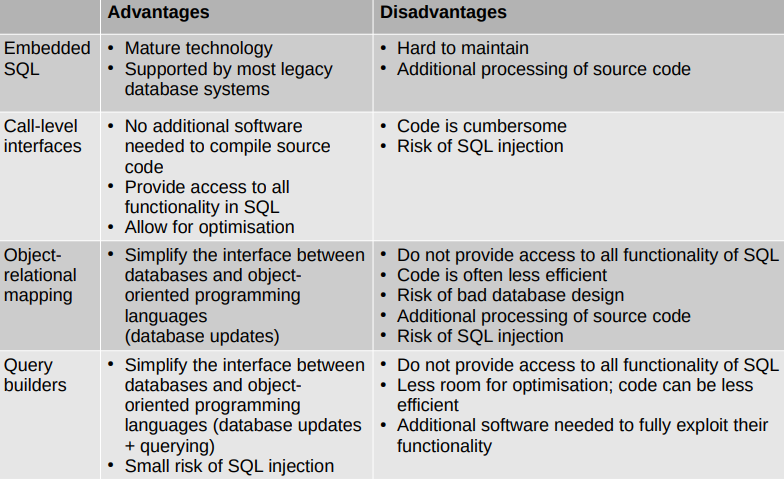
\includegraphics[width=\textwidth,keepaspectratio]{prog_pros_cons}
\end{figure}

\chapter{Concurrency \& Recovery}

Allow a number of different clients/computers/computers programs access to the same database.

\section{Concurrency in SQLite}

\begin{itemize}
    \item SQLite is a simple program that stores a database in one file on disk
    \item It does not manage network access
    \item Distributed approach possible: put .db file on file sharing server
\end{itemize}

\begin{minipage}{0.48\textwidth}
\textred{Disadvantages of relying on a file server} :

When one client has write access to the database file, no other client can have either read or write access $\rightarrow$ Bad performance
\end{minipage}
\hfill
\begin{minipage}{0.48\textwidth}
\textgreen{Solution} :
\begin{itemize}
    \item Client sends SQL statement to the server
    \item Each client sends \textit{transactions}
    \item Server sends results to the client
\end{itemize}
\end{minipage}

The database management statement should execute the transaction in a manner that is \textblue{ACID}. We need a scheduler to know wich task to execute first.

\subsection{Simplest Schedule : Serial Execution}

\begin{itemize}
    \item FIFO : each transaction is executed entirely before executing the next one
    \item Disadvantage : long waiting times
\end{itemize}

\subsection{Recoverable Schedules}

\begin{itemize}
    \item Databases should support \textblue{rollback} : undoing the operations of a transaction
    \item Databases should have \textblue{recoverable schedules} : schedules in which the database system would never have to rollback a transaction for which the commit request has been confirmed
    \item Solution : only commit a transaction if all transactions from which it has read modified data have commited to avoid cascading rollbacks (when one rollback leads to another rollback)
    \begin{figure}[H]
        \centering
        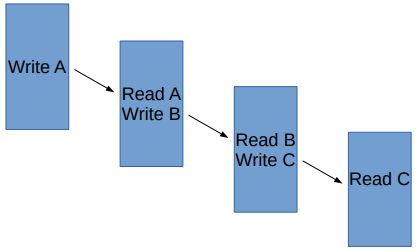
\includegraphics[height=3.5cm,keepaspectratio]{recoverable_schedules}
    \end{figure}
\end{itemize}

\subsection{Locking}

\begin{itemize}
    \item Used to avoid reading/writing when it should not happen
    \item The most popular type of lock is shared/exclusive (or read/write) lock
    \item Every data item (i.e. block or record) has a lock that can take three states, and operations that can change the state :
\end{itemize}

\begin{minipage}[t]{0.48\textwidth}
    \textblue{unlocked}, using the operation unlock(X)
    \begin{figure}[H]
        \centering
        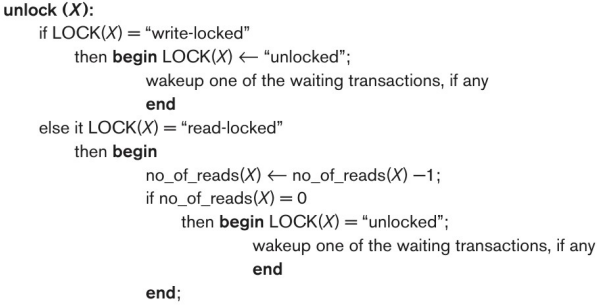
\includegraphics[width=\textwidth,keepaspectratio]{unlock}
    \end{figure}
\end{minipage}
\hfill
\begin{minipage}[t]{0.48\textwidth}
    \textblue{read-locked}, using the operation read\_lock(X)
    \begin{figure}[H]
        \centering
        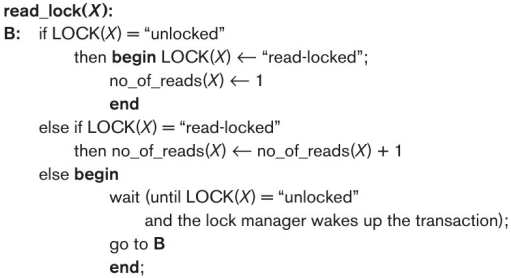
\includegraphics[width=\textwidth,keepaspectratio]{read_lock}
    \end{figure}
\end{minipage}
\begin{center}
    \begin{minipage}[t]{0.48\textwidth}
        \textblue{write-locked}, using the operation write\_lock(X)
        \begin{figure}[H]
            \centering
            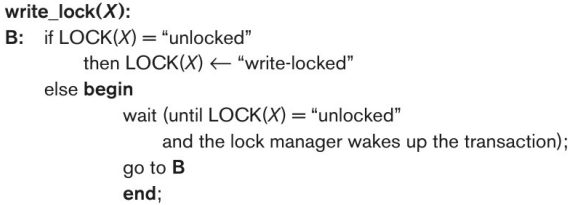
\includegraphics[width=\textwidth,keepaspectratio]{write_lock}
        \end{figure}
    \end{minipage}
\end{center}

\begin{itemize}
    \item Before we read an item, we request a read lock; before we write an item, we request a write lock
    \item If an item is locked, we are limited in what we can do
\end{itemize}

\subsubsection{Naïve Lock/Unlock}

\begin{itemize}
    \item Add locking statements immediately before and after reads and writes
    \item Problem :
    \begin{figure}[H]
        \centering
        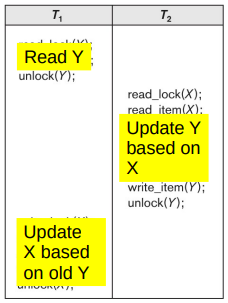
\includegraphics[height=4cm,keepaspectratio]{naive_pb}
    \end{figure}
\end{itemize}

\subsubsection{Two-Phase Locking Protocol}

\begin{itemize}
    \item Simplest approach to avoid an execution that is not serializable
    \item Requires that all lock statements are put before all unlock statement.
    \item Problem : can lead to deadlocks
\end{itemize}

\subsubsection{Deadlocks : Solutions}

\begin{itemize}
    \item \textblue{Conservative 2PL} : Transaction declares all read/writes locks at the beginning of the transaction, and receives all locks at the same time (Simple, but inefficient : items are locked that may not be needed yet)
    \item \textblue{Time-out} : abort a transaction when its waiting too long (most commonly used approach)
    \item \textblue{Deadlock detection} ; create a waiting-for graph and determine whether the graph has cycle (could be time-consuming if run for every lock; uses other heuristics)
\end{itemize}

\section{Failure Recovery}

\begin{itemize}
    \item \textblue{Aims} : recover for failure while ensuring ACID
    \item Different type of failures : Hard disk crash, power interruption, constraint violation, transaction abort
\end{itemize}

\subsection{Log files}

\textblue{Goal} : keep track of the operations of a transaction in a log file on disk.

Different types of logs :

\subsubsection{Undo Log}

Before data is written to disk, the old value of the data is written to a log file.

\begin{figure}[H]
    \centering
    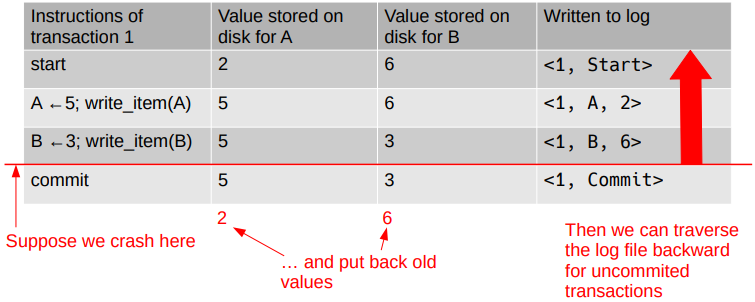
\includegraphics[width=0.7\textwidth,keepaspectratio]{undo_log}
\end{figure}

\begin{minipage}{0.48\textwidth}
\textgreen{Advantages} :
\begin{itemize}
    \item Idempotent: if the recovery process crashes, one can just start it again
    \item Simple: data is written immediately to disk, where other programs can retrieve it
\end{itemize}
\end{minipage}
\hfill
\begin{minipage}{0.48\textwidth}
\textred{Disadvantages} :
\begin{itemize}
    \item Potentially inefficient to write every\\tiny change to disk immediately (consider many writes to the same block)
\end{itemize}
\end{minipage}

\paragraph{Undo Log : caching}

Writing on cache to avoid writing every time on the disk

\begin{itemize}
    \item We cannot commit a transaction before it is written to disk (otherwise we may still lose its content)
    \item If there are many small transactions, there are two possibilities :
    \begin{itemize}
        \item Delay finishing them (confirming commit) till they are all written to disk in a cache flush
        \item Write them to disk sooner
    \end{itemize}
    \item In both cases there is still performance degradation
\end{itemize}

\subsubsection{Redo Log}

\textblue{Goal} : Write changes to the log file on disk when a commit is confirmed, but reflect the changes on disk only later when emptying caches.

\begin{figure}[H]
    \centering
    \includegraphics[width=0.65\textwidth,keepaspectratio]{redo_log}
\end{figure}

\begin{minipage}{0.48\textwidth}
\textgreen{Advantages} :
\begin{itemize}
    \item Faster database operation: the database operates mostly from main memory (still, log files are updated when a transaction ends)
\end{itemize}
\end{minipage}
\hfill
\begin{minipage}{0.48\textwidth}
\textred{Disadvantages} :
\begin{itemize}
    \item As we can only update data on disk after a commit, what do we do with large transactions? (e.g., Transactions that don’t fit in memory; too many items in the data affected)
\end{itemize}
\end{minipage}

\subsubsection{Undo/Redo Log}

\begin{itemize}
    \item Write both old and new values to the log
    \item For transactions that are not finished, the "old" values in the log are used to undo any changes that may have been written to disk already
    \item For transactions that are finished, the "new" values in the log are used to redo any changes that may have not been written to disk yet
\end{itemize}

\begin{minipage}{0.48\textwidth}
    \begin{figure}[H]
        \centering
        \includegraphics[width=\textwidth,keepaspectratio]{undo_redo_1}
    \end{figure}
\end{minipage}
\hfill
\begin{minipage}{0.48\textwidth}
    \begin{figure}[H]
        \centering
        \includegraphics[width=\textwidth,keepaspectratio]{undo_redo_2}
    \end{figure}
\end{minipage}

\subsubsection{Conclusion}

\begin{itemize}
    \item Ensuring ACID properties requires maintaining a log file (journal) on disk
    \item Performance tuning :
    \begin{itemize}
        \item Put the log file on a faster type of disk
        \item Tuning of the log file: how often are caches flushed, how often do we clean up the log file, checkpoints
    \end{itemize}
    \item Downsides :
    \begin{itemize}
        \item Maintaining a log file takes time
        \item A log file takes additional space
    \end{itemize}
\end{itemize}

\chapter{NoSQL}

NoSQL = "Not Only SQL"


\begin{itemize}
    \item \textblue{Motivations for NoSQL} :
    \begin{itemize}
        \item \textblue{Scalability} : relational databases do not scale to the size of data that needs to be maintained by Google, Facebook, Amazon, ...
        \item \textblue{Supported data types and data queries} : social networks, webpages, documents are not easily stored and queried using Relational Database Management Systems
    \end{itemize}        
    \item Examples :
    \begin{itemize}
        \item \textblue{Semi-structured data} : data that has structure, but does have a fixed schema; the data is often stored in a textual document and describes its own structure (JSON file, ...)
        \item \textblue{Network data} : structures consisting of labeled nodes and edges (social networks, biological networks, communication networks, ...)
        \item \textblue{Other data} : Image, video, ...
    \end{itemize}
\end{itemize}

\section{Types Of NoSQL Databases}

\subsection{Graph Databases}

\textblue{Neo4J and Cypher}

\begin{itemize}
    \item An ACID database (just like relational databases)
    \item Assumes a labeled property graph data model
\end{itemize}

\begin{figure}[H]
    \centering
    \includegraphics[width=0.7\textwidth,keepaspectratio]{neo4j}
\end{figure}

\subsection{Key-Value Stores}

Two scaling problems to consider :
\begin{enumerate}
    \item Scaling towards \textblue{large numbers of users}
    \begin{itemize}
        \item To reduce response times, servers should be physically close to users
        \item Data needs to be replicated on multiple machines
    \end{itemize}
    \item Scaling towards \textblue{large amounts of data}
    \begin{itemize}
        \item Storing all data on one machine is not feasible
        \item Data needs to be distributed across multiple machines
    \end{itemize}
\end{enumerate}

\subsubsection{Replication}

The same data is store on multiple servers
\begin{itemize}
    \item Be able to recover from errors
    \item Provide shorter response times to different user
\end{itemize}

\subsubsection{Partitioning}

Data is too large, is stored on multiple servers
\begin{itemize}
    \item Horizontal partioning / Sharding
    \item Vertical partioning
\end{itemize}

\subsection{Capt Theorem}

The CAP theorem, also known as Brewer's theorem, states that in a distributed computer system, it is impossible to simultaneously achieve all the following three guarantees: consistency, availability, and partition tolerance.

\begin{itemize}
    \item \textblue{Consistency} refers to every read operation receiving the most recent write or an error. In other words, all nodes in the distributed system see the same data at the same time.
    \item \textblue{Availability} means that every request to the system receives a response, even in the presence of failures. THe system remains operational and accessible to users.
    \item \textblue{Partition} tolerance ensures that the system continues to function and provide availability even if network partitions occure, causing messages to be delayed or lost between nodes.
\end{itemize}

The CAP theorem states that in the event of a network partition, a distributed system must choose between maintaining consistency (C) or availability (A). It is not possible to have both guarantees simultaneously. However, partition tolerance (P) is a necessary characteristic for a distributed system.

\begin{figure}[H]
    \centering
    \includegraphics[width=0.55\textwidth,keepaspectratio]{cap}
\end{figure}

In practical terms, the CAP theorem implies that when designing distributed systems, trade-offs must be made between consistency and availability based on the specific requirements and constraints of the application and its environment. Different systems prioritize either consistency or availability, leading to different consistency models (such as strong consistency or eventual consistency) and availability strategies (such as high availability or fault tolerance).

So Instead of ACID semantics, many NoSQL database systems provide \textblue{BASE} semantics:

\begin{itemize}
    \item \textblue{Basically Available} : the system remains available even if a part stops working
    \item \textblue{Soft state} : the same data item may be in a different state in different parts of the system
    \item \textblue{Eventual consistency} : within finite time after a set of write operations (but not necessarily immediately) all data items will be in the state reflected by the last write to them
\end{itemize}

\section{Key-Value Stores}

Distributed database systems that for a given key can quickly retrieve associated data, or update associated data.

\subsection{Documents stores}

\begin{itemize}
    \item Store semi-structured documents
    \item Provide support for processing these structures documents
    \item Typically provide \textit{horizontal partitioning} (sharding)
\end{itemize}

\subsubsection{MongoDB}

Has a querying interface, but this querying interface is focused on retreiving from \textit{one document} collection those documents satisfying conditions.

A time-consuming linear scan is needed for queries that access other attributes than the key, unless indexes are maintained.

\begin{itemize}
    \item Distributed nature
    \begin{itemize}
        \item The same document can be stored on multiple servers (\textit{replication})
        \item The documents within the same collection can be stored across multiple servers if the collection is too large (\textit{sharding})
    \end{itemize}
    \item By default
    \begin{itemize}
        \item For every document there is \textit{one} primary server: all \textit{write} operations for that document are directed towards that server
        \item \textit{Read/write} operations to the primary server are \textit{immediately consistent}
        \item \textit{Read} operations can also be served by any other server storing the document, but they are only \textit{eventually consistent}
        \item There can be an even number of secondary servers that store copies of the document
        \item If the primary server fails, the secondary servers organize an \textit{election} to appoint one of them as the new primary server
    \end{itemize}
\end{itemize}

\subsubsection{CouchDB}

\begin{itemize}
    \item AP document store instead of CP document store
    \item All replicas can process a write request
    \begin{itemize}
        \item Increase availability in case of a partition
        \item Decreases consistency in case of a partition
    \end{itemize}
    \item Versioning : every server maintains a history of changes, which will be eventually consistent
\end{itemize}

\subsection{Generic Key-Value Stores}

\subsubsection{Amazon DynamoDB}

Commercial product to store data in Amazon's cloud. Consists of tables :
\begin{itemize}
    \item Within a table is stored a set of items
    \item Each items consist of a set of (attribute, value) pairs
    \item Every table must have one attribute that servers as its key, and this attribute must be present in all items
\end{itemize}

\newpage
Withing a table, DynamoDB can quickly retrieve the corresponding item for a given key, and the value for a given attribute within that item
\begin{itemize}
    \item Items are shared (horizontally partitioned)
    \item No query language, only a interface for retrieving values for a given (table, key, attribute)
    \item Distributes :
    \begin{itemize}
        \item Eventual consistency
        \item No primary server, multiple nodes may process writes
        \item Versioning to reconcile
        \item Similar open source products (LinkedIn's Voldemort, Redis, ... $\rightarrow$ focus in keeping data in memory)
    \end{itemize}
\end{itemize}

\subsection{Column Stores}

Suppose we have columns in our data (A, B, C, D) and we are looking for documents with a given value in column D.

\begin{figure}[H]
    \centering
    \includegraphics[width=0.55\textwidth,keepaspectratio]{wide_column}
\end{figure}

\subsubsection{Apache HBase}

\begin{itemize}
    \item A database in HBase consists of \textit{tables}
    \item Within a table is stored a set of \textit{items}
    \item Each \textit{item} consists of a set of (column family, column quantifier, value) tuples
    \begin{itemize}
        \item Column Families are specified when the table is created
        \item Column Quantifiers are not fixed in advance : the data is still self-describing, as within a column family any nymber of attributes quantifiers is possible
    \end{itemize}
    \item Every \textit{item} has a \textit{key} that uniquely identifies the item within the table, and which \textit{has an order}
    \begin{itemize}
        \item The order is used in sharding : shards consist of consecutive keys
    \end{itemize}
\end{itemize}

\begin{center}
\begin{tabular}{|l|l|l|}
\hline 
  & HBase & Cassandra \\ 
\hline 
Locking server & One server for locking & Multiple locking server \\ 
\hline 
Consistency & High & Low \\ 
\hline 
Availability & Low & High \\ 
\hline 
\end{tabular} 
\end{center}

For both, when a server fails, one of the remaining servers will take over.

\paragraph{Hadoop File System (HDFS)}

\begin{itemize}
    \item Implements a distributed file system
    \item Programs can red and writes files to the file system
    \item Files have a path
    \item HDFS has one NameNode that locates files, processes requests for adding/removing/moving files
    \begin{figure}[H]
        \centering
        \includegraphics[width=0.55\textwidth,keepaspectratio]{hdfs}
    \end{figure}
    \begin{itemize}
        \item Single point of failure; lower availability
    \end{itemize}
    \item The number of files that can be stored in the HDFS is "limited" (400 million files)
\end{itemize}

\paragraph{Apach Hadoop (MapReduce)}

\begin{itemize}
    \item \textblue{Map} map$(k1, v1) \rightarrow$ list$(k2, v2)$ : a function that returns for a key and its value, a new list of (key, values) pairs
    \item \textblue{Reduce} reduce$(k2,$ list$(v1)) \rightarrow$ list$(v3)$ : a function that returns for a key and a list of values, a new list of values
\end{itemize}

\subsubsection{Apache Hive}

Provides an SQL-like interface to tables stored in the HDFS and calculates answers to queries using Hadoop/MapReduce. Its original purpose is to answer queries that \textit{read} data on a massive scale.

\begin{itemize}
    \item If was originally \textit{not} designed to support online transactions efficiently
    \item But developers are increasingly adding ACID support
    \item Currently ACID at a row-level, using locks for rows on appropriate data formats.
\end{itemize}

Queries are transformed into relational algebra, operators are implemented using Map \& Reduce (limited query optimization)

\subsubsection{Apache Hive vs Apache HBase}

\begin{itemize}
    \item Apache HBase is a key-value store that supports high frequency read/writes; can be used to support a live running system
    \item Apache Hive is meant to be used by analysts that have collected large amounts of data and wish to run queries over that data
\end{itemize}

\newpage
\subsubsection{Apache Spark SQL}

\begin{itemize}
    \item Data processing framework based on \textit{Resilient Distributed Datases (RDDs)}, datasets that are (temporarily) stored in the memory of distributed servers
    \begin{figure}[H]
        \centering
        \includegraphics[width=0.6\textwidth,keepaspectratio]{apache_spark}
    \end{figure}
    \item Support Map, Reduce, and other operations
    \item Implementation of SQL on Spark
\end{itemize}

\subsubsection{Apache Spark SQL vs Apache Hive}

\begin{itemize}
    \item Spark SQL relies on Spark, which supports in-memory data structures $\rightarrow$ better performance
    \item Spark SQL supports a wider range of input data formats, including all data formats supported by Hive
    \item Apache Hive is more mature, and is adding support for transactions $\rightarrow$ starts to be more usable as a database system
\end{itemize}

\subsubsection{NewSQL: Google Spanner Features}

\begin{itemize}
    \item Relational data model, support for standard SQL, ACID
    \item Software as a service; an entirely private world-wide network is used to ensure high availability
    \begin{itemize}
        \item A clock is used to ensure every read/write request, and every data item, has a reliable time stamp with bounded error
        \item Multiple versions of a data item are maintained
        \item Replicas return an older version as long as a write request is not committed (time stamp read < time stamp write commit)
        \item High concistency: writes are only confirmed if all nodes worldwide have confirmed that they have processed the write
    \end{itemize}
\end{itemize}
